\documentclass[12pt,a4paper]{article}

\usepackage{color}
\usepackage{amsxtra}  
\usepackage{amsthm}
\usepackage{amssymb}
\usepackage{amsfonts}
\usepackage{graphicx}  
\usepackage{rotating}


\begin{document}

\title{Dynamics of pinned polymer loop in 1D}
\author{Wenwen Huang}
\date{\today}

\maketitle

\section{Model}
\label{sec:model}
Polymer dynamics of bead rod can be mapped to particle hopping model by the
coarse grain that rod orientation be either right$(+1)$ or left$(-1)$. This
binary state of rods can be represented by the state of lattice sites which is
either occupied by one particle$(1)$ or empty$(0)$. Denote the state of
$i^{th}$ rod by $z_i$ and state of $i^{th}$ lattice site by $s_i$, then we have
$s_i = (z_i + 1)/2$.

It is easy to show that the configuration of polymer can be one to one mapped to
the configuration of lattices with particles. The dynamics of be polymer then
can be investigated in the context of particle hopping process, known as ASEP.
Here we consider the case of pinned polymer loop model in an external force
field which corresponds to $N$ particles hopping in $2N$ lattices sites with
reflecting boundaries. Other models, e.g. free bead rod chain, corresponds to
simply different settings of ASEP will be discussed in our future work.  

To calibrate dynamics of bead rod and ASEP, we need to know exactly what is the
correspondence of a single particle hopping step to left or right. This is
illustrated in the sketch Fig. \ref{fig:calibration}

One single hopping step of a particle affects two neighbouring lattice sites,
namely two neighbouring rods orientation. The switch of the site state
corresponds to flip of the rod orientation. With this intuition, it is easy to
understand that one hopping step of a particle is equivalent to two neighbouring
rods rotate for $\pi$, i.e. a flip. Notice that a flip of two neighbouring
rods means that the shared bead diffuse for a distance of $2a$, where $a$ is
the length of rod. We use this to estimate the time scale of the dynamics.
Denote $\tau_0$ the time of a particle hopping step,  then 
\begin{equation}
    \label{eq:time_scale}
    \tau_0 \propto \frac{4a^2}{2D_0} = \frac{2a^2\xi}{k_B T}
\end{equation}
where $D_0$ is the diffusion coefficient of the bead, $\xi$ is friction
coefficient, $k_B$ is Boltzmann factor, and $T$ is temperature.

Next, we need to know what is the effect of force exerting on beads to the
hopping of particles. Force changes the bias of rod flipping thus the bias of
particle hopping. Denote $\alpha$, $\beta$ the rate of particle hopping to left
and right, respectively. We have
\begin{equation}
    \label{eq:detailed_balance}
    \beta / \alpha = \exp(-\frac{\Delta E}{k_B T})
\end{equation}
where $\Delta E$ is the energy difference between the two configuration before
and after hopping. Without lose of generality we assume the constant force $F$
exerting on beads is in the direction of right. So we have $\Delta E = 2Fa$.

On the other hand, the totally rate of hopping is irrelevant with the external
force but depends on the temperature. Actually this can be obtained from the
hopping time scale Eq. \eqref{eq:time_scale}. We thus have
\begin{equation}
    \label{eq:total_rate}
    \alpha + \beta = r_{total} = 1/\tau_0
\end{equation}

With Eq. \eqref{eq:detailed_balance} and Eq. \eqref{eq:total_rate}, we can
solve the hopping rates $\alpha$ and $\beta$. 
\begin{subequations}
    \label{eq:alpha_beta}
    \begin{equation}
        \alpha  =  \frac{r_{\text{total}}}{1+\exp{(-2Fa / k_B T)}}
    \end{equation}
    \begin{equation}
        \beta  =   \frac{r_{\text{total}}\exp{(-2Fa / k_B T)}}{1+\exp{(-2Fa / k_B
                T)}} \\
    \end{equation}
\end{subequations}

Now we have a welled defined ASEP model corresponds to the dynamics of pinned
bead rod polymer loop in external force field.
In order to solve the dynamics, let us discuss more about the \emph{pseudo}
particles in the mapped ASEP model. The dynamics of these \emph{pseudo} particles
is essentially Brownian particles with constant drift. Without loss of
generality, we set the lattice constant which denotes the width of lattice site
to $1$. Then the diffusivity and drifting velocity of the \emph{pseudo} particle
$D$ and
$\mu$ can be written as 
\begin{subequations}
    \label{eq:diffusivity_drift}
    \begin{equation}
        D  =  1^2/2\tau_0 = \frac{1}{2}(\alpha + \beta)
    \end{equation}
    \begin{equation}
        \mu = \alpha - \beta
    \end{equation}
\end{subequations}

The dynamical equation of the particle system can be describe by Fokker-Planck
Equation 
\begin{equation}
\begin{aligned}
    \label{eq:fp}
    \frac{\partial p(\mathbf{x}, t | \mathbf{x}_0)}{\partial t} = & D \left(
        \frac{\partial^2}{\partial x_1^2} + \frac{\partial^2}{\partial x_2^2} +
        \cdots+\frac{\partial^2}{\partial x_N^2}\right)p(\mathbf{x},t|\mathbf{x}_0) \\ 
    & - \mu\left(\frac{\partial}{\partial x_1} +
        \frac{\partial}{\partial x_2} + \cdots + \frac{\partial}{\partial x_N}
    \right) p(\mathbf{x}, t | \mathbf{x}_0) 
\end{aligned}
\end{equation}
where $\mathbf{x}=(x_1, x_2, \cdots, x_N)^T$ is the vector denotes the position
of each particle and $\mathbf{x_0}$ denotes the initial position of particles.
In general case $D$ and $\mu$ can depend on time and position. However, what
we consider here $D$ and $\mu$ are just constants.
The reflecting boundary conditions of the ASEP system can be written as
\begin{subequations}
    \label{eq:reflecting_boundary}
    \begin{equation}
        \left(D\frac{\partial}{\partial x_1}p(\mathbf{x},t|\mathbf{x}_0) 
            -\mu p(\mathbf{x},t|\mathbf{x}_0)\right) \Bigg|_{x_1=0} = 0
    \end{equation}
    \begin{equation}
        \left(D\frac{\partial}{\partial x_N}p(\mathbf{x},t|\mathbf{x}_0) 
            -\mu p(\mathbf{x},t|\mathbf{x}_0)\right) \Bigg|_{x_N=L} = 0
    \end{equation}
\end{subequations}
Where $L=2N$ in our case. Furthermore, notice the exclusive condition which
means particle can not overtake each other. This can be formulated as follow
\begin{equation}
    \label{eq:exclusive_condition}
    \left(\frac{\partial}{\partial x_{i+1}}p(\mathbf{x},t|\mathbf{x}_0) -
        \frac{\partial}{\partial x_{i}} p(\mathbf{x},t|\mathbf{x}_0)
    \right)\Bigg|_{x_{i}=x_{i+1}} = 0 
\end{equation}
Finally, the initial condition we assume is
\begin{equation}
    \label{eq:initial_condition}
    p(\mathbf{x}, 0 | \mathbf{x}_0) =
    \delta(x_1-x_{1,0})\delta(x_2-x_{2,0})\cdots\delta(x_N-x_{N,0})
\end{equation}

\section{Solution}
\label{sec:solution}
The solution of Eq. \eqref{eq:fp} together with Eq.
\eqref{eq:reflecting_boundary},\eqref{eq:exclusive_condition},\eqref{eq:initial_condition}
can be found by coordinate Bethe Ansatz\cite{}.  We assume the solution of
$p(\mathbf{x}, t | \mathbf{x}_0)$ can be written in the following form
\begin{equation}
    \label{eq:pdf_solution}
    p(\mathbf{x}, t | \mathbf{x}_0) = \sum_{\sigma\in
        S_{N}}{\psi(x_1, x_{\sigma(1)};t)\psi(x_2, x_{\sigma(2)};t)\cdots\psi(x_N,
        x_{\sigma(N)};t)}
\end{equation}
where $\sigma$ is a $N$-permutation of $x_{i,0}$. This means the expanded form
of Eq. \eqref{eq:pdf_solution} reads
\begin{align*}
    \label{eq:pdf_solution_expanded}
    p(\mathbf{x}, t | \mathbf{x}_0) = &
    {\psi(x_1, x_{1,0};t)\psi(x_2, x_{2,0};t)\cdots\psi(x_N,x_{N,0};t)} + \\
    & {\psi(x_1, x_{2,0};t)\psi(x_2, x_{1,0};t)\cdots\psi(x_N,x_{N,0};t)} + \\
    & \text{ all other permutations of } \{x_{1,0}, x_{2,0}, \cdots, x_{N,0}\}
\end{align*}
After that, it is important to find out the correct $\psi(x_i,
x_{\sigma(i)};t)$.  Surprisely, we will show here that $\psi(x_i,
x_{\sigma(i)};t)$ is simply the form of one single Brownian particle with
drifting in the reflecting box. But before dive into the derivation, we want to
point out Eq. \eqref{eq:pdf_solution} is not a common Bethe Ansatz solution of a
1D $N$-particle system, e.g. it is not the solution form when the boundary is
periodic or open\cite{}. The key reason it works in this case is rooting from
the reflecting boundaries of the system. Because of the reflecting boundaries,
the response of particles in the middle or in the periphery will be exactly the
same, i.e. reflecting. This leads to a factorized form of the $N$-particle
PDF, i.e. Eq. \eqref{eq:pdf_solution}. In other words, Eq.
\eqref{eq:pdf_solution} is the solution of the 1D $N$-particle system as long as
the boundary is reflecting, even through the external field is much more complex
than the constant one we considered in this work. We will give a proof that can
easily extend to more general cases in the following text.

The proof that Eq. \eqref{eq:pdf_solution} is indeed a solution is actually
quite simple and straight forward. Notice that $\psi(x_i, x_{j,0};t)$ is the
solution of single particle drifting in the box so that

\begin{subequations}
\label{eq:single_particle}
\begin{equation}
    \label{eq:single_particle_1}
    \frac{\partial \psi(x_i, x_{j,0};t)}{\partial t} =
    D \frac{\partial^2}{\partial x_i^2} \psi(x_i, x_{j,0};t) - 
    \mu\frac{\partial}{\partial x_i}\psi(x_i, x_{j,0};t)
\end{equation}
\begin{equation}
    \label{eq:single_particle_2}
    \left(D\frac{\partial}{\partial x_i}\psi(x_i, x_{j,0};t)
        - \mu\psi(x_i, x_{j,0};t)\right) \Bigg|_{x_i=0} = 0
\end{equation}
\begin{equation}
    \label{eq:single_particle_3}
    \left(D\frac{\partial}{\partial x_i}\psi(x_i, x_{j,0};t)
        - \mu\psi(x_i, x_{j,0};t)\right) \Bigg|_{x_i=L} = 0
\end{equation}
\begin{equation}
    \label{eq:single_particle_4}
    \psi(x_i, x_{j,0};0) = \delta(x_i-x_{j,0})
\end{equation}
\end{subequations}

We firstly exam that Eq. \eqref{eq:pdf_solution} satisfies the Fokker-Planck
equation. Just substitute Eq. \eqref{eq:pdf_solution} into Eq. \eqref{eq:fp} we
obtain
\begin{align*}
    % \label{eq:proof_fp}
    \text{lhs} & = \sum_{\sigma\in
        S_N}\sum_{i=1}^N\frac{\partial\psi(x_i,x_{\sigma(i)};t)} {\partial
        t}\prod_{j\neq i}\psi(x_j, x_{\sigma(j)};t) \\
    \text{rhs} & = \sum_{\sigma\in
        S_N}\sum_{i=1}^N\left(D\frac{\partial^2\psi(x_i,
            x_{\sigma(i)};t)}{\partial x_i^2} - \mu\frac{\partial\psi(x_i,
            x_{\sigma(i)};t)}{\partial x_i}\right)\prod_{j\neq i}
    \psi(x_j, x_{\sigma(j)};t)
\end{align*}
It is obvious that $\emph{lhs} = \emph{rhs}$ because of Eq.
\eqref{eq:single_particle_1}. And other permutation terms of Eq.
\eqref{sec:solution} can be proved in the same way.

Next, we show that the reflecting boundary conditions is satisfied, again just
plug Eq. \eqref{eq:pdf_solution} into Eq. \eqref{eq:reflecting_boundary}, obtain
\begin{align*}
    \label{eq:proof_boundary}
    & \left(D\frac{\partial}{\partial x_1}p(\mathbf{x},t|\mathbf{x}_0)
         - \mu p(\mathbf{x},t|\mathbf{x}_0) \right)\Bigg|_{x_1=0} \\
     & = \sum_{\sigma\in S_N}\left(D\frac{\partial\psi(x_1, x_{\sigma(1)};t)}
        {\partial x_1} - \mu \psi(x_1, x_{\sigma(1)};t)
        \right)\prod_{j\neq 1}\psi(x_j, x_{\sigma(j)};t) \Bigg|_{x_1 = 0} \\
    & = 0
\end{align*}
Eq. \eqref{eq:single_particle_2} is ultilized for the last step. Similarly, the
boundary condition at $x_N = L$ is also satisfied because of Eq.
\eqref{eq:single_particle_3}.

We then show that the exclusive condition Eq. \eqref{eq:exclusive_condition}
is also true. Take a pair of permutation terms that we can always find in the
solution of Eq. \eqref{eq:pdf_solution}, 
\begin{align*}
    \phi = & \psi(x_i, x_{m,0};t)\psi(x_{i+1}, x_{n,0};t)
    \prod_{j\neq i,i+1} \psi(x_j, x_{\sigma(j)};t)  \\
    & + \psi(x_i, x_{n,0};t)\psi(x_{i+1}, x_{m,0};t)\prod_{j\neq i,i+1} 
    \psi(x_j, x_{\sigma(j)};t)
\end{align*}
It is easy to verify that
\begin{align*}
    % \label{eq:proof_exclusive}
    \left(\frac{\partial \phi}{\partial x_{i+1}} - \frac{\partial \phi}{\partial
            x_{i}}\right)\Bigg|_{x_i = x_{i+1}} & =  
    \left(\frac{\partial\psi(x_{i+1}, x_{m,0};t)}{\partial x_{i+1}}\psi(x_{i},
        x_{n,0};t) + \frac{\partial\psi(x_{i+1}, x_{n,0};t)}{\partial
            x_{i+1}}\psi(x_{i}, x_{m,0};t)\right. \\ 
    &\left. - \frac{\partial\psi(x_i, x_{m,0};t)}{\partial x_i}\psi(x_{i+1},
        x_{n,0};t) - \frac{\partial\psi(x_i, x_{n,0};t)}{\partial
            x_i}\psi(x_{i+1}, x_{m,0};t)\right) \\ 
    & \times\prod_{j\neq i,i+1}\psi(x_j, x_{\sigma(j)};t)\Bigg|_{x_i = x_{i+1}} \\
    & = 0 
\end{align*}
And because $p(\mathbf{x}, t | \mathbf{x_0})$ can be written as the summation of
$\phi$, so the exclusive condition Eq. \eqref{eq:exclusive_condition} is proved.

Last, we come to the initial condition. Simply plug Eq.
\eqref{eq:single_particle_4} into the solution Eq. \eqref{eq:pdf_solution} we get
\begin{align*}
    % \label{eq:proof_initial}
    p(\mathbf{x}, 0 | \mathbf{x}_0) = & 
    \delta(x_1-x_{1,0})\delta(x_2-x_{2,0})\cdots\delta(x_N-x_{N,0}) \\
    & + \delta(x_1-x_{2,0})\delta(x_2-x_{1,0})\cdots\delta(x_N-x_{N,0}) \\
    & \text{ all other permutations of } \{x_{1,0}, x_{2,0}, \cdots, x_{N,0}\}
\end{align*}
All the other terms vanish except the first in the above equation because by
definition we have $x_{1}<x_{2}<\cdots<x_{N}$ and $x_{1,0}<x_{2,0}<\cdots<x_{N,0}$.  
We thus prove the initial condition Eq. \eqref{eq:initial_condition}. And now we
finally proved that Eq. \eqref{eq:pdf_solution} with $\psi(x_i, x_{j,0};t)$
satisfies Eq.  \eqref{eq:single_particle} is the solution of our problem.
Notice that this procedure of proof is still valid in the case that external
field is more complex than just constant.

Now let us come back to the solution Eq. \eqref{eq:pdf_solution}. So if we know
the exact form of $\psi(x_i,x_{j,0};t)$ then we have a close form solution of
our problem. Luckly, $\psi(x_i,x_{j,0};t)$ is known thanks to the recent works\cite{}.
In our notation, $\psi(x_i,x_{j,0};t)$ can be written as
\begin{equation}
    \label{eq:single_particle_solution}
    \psi(x_i,x_{j,0};t) = \psi_0(x_{i}) + \sum_{n=1}^\infty\exp(-\lambda_n
    t)\varphi_n(x_{i}, x_{j,0})
\end{equation}
where $\psi_0(x_{i})$ is stationary state PDF that irrelevant with time and
initial condition. $\lambda_n$ is the eigenvalue related to $n^{th}$
relaxation mode, $\varphi_n(x_i, x_{j,0})$ is the function relates to initial
condition. These terms can be written as following
\begin{subequations}
    \label{eq:single_particle_solution_terms}
    \begin{equation}
        \psi_0(x_i) = \left\{\begin{array}{ccl} \frac{1}{L} & \mbox{for} & \mu=0 \\
                \frac{\mu}{D}\frac{\exp(\frac{\mu x_i}{D})}{\exp(\frac{\mu L}{D})-1}
                    & \mbox{for} & \mu\neq 0 \end{array}\right.
    \end{equation}
    \begin{equation}
        \lambda_n = \frac{\mu^2}{4D} + \frac{Dn^2\pi^2}{L^2}
    \end{equation}
    \begin{equation}
        \varphi_n(x_i, x_{j,0}) =
        \frac{D\pi^2\exp(\frac{\mu}{2D}(x_i-x_{j,0}))}{2\lambda_n L}X_n(x_i)
        X_n(x_{j,0})
    \end{equation}
    \begin{equation}
        X_n(x) = \frac{2n}{L}\cos(\frac{n\pi x}{L}) + \frac{\mu}{D\pi}\sin(\frac{n\pi x}{L})
    \end{equation}
\end{subequations}

Plug Eq.
\eqref{eq:single_particle_solution}\eqref{eq:single_particle_solution_terms}
into Eq. \eqref{eq:pdf_solution} we get the close form $N$-particle PDF.
However, it is so lengthy that not clean enough for us to understand the
physics. Notice what we usually interested in are the stationary state and the
longest relaxation time. So we keep only these two terms after the
substitution, obtain

\begin{equation}
    \label{eq:p0_p1}
    p(\mathbf{x}, t | \mathbf{x}_0) = p_0(\mathbf{x}) + p_1(\mathbf{x}, t|
    \mathbf{x}_0) + p_H(\mathbf{x}, t|\mathbf{x}_0)
\end{equation}
where $p_H$ is the summation of all higher mode terms $n>1$, $p_0$ and $p_1$
are stationary mode and longest relaxation mode, respectively, which reads
\begin{subequations}
    \label{eq:pdf_terms}
    \begin{equation}
        p_0(\mathbf{x}) = N!\,\psi_0(x_1)\prod_{i=1}^{N-1}\psi_0(x_{i+1})\Theta(x_{i+1}-x_{i})
    \end{equation}
    \begin{equation}
        p_1(\mathbf{x}, t| \mathbf{x}_0) =
        A_1(\mathbf{x}, \mathbf{x}_0)\exp(-\lambda_1 t)
    \end{equation}
    \begin{equation}
        A_1(\mathbf{x}, \mathbf{x}_0) = 
        (N-1)!\,\sum_{i=1}^N\psi_0(x_i)\sum_{j\neq i}^N 
        \sum_{k=1}^N\varphi_1(x_j,x_{k,0})
    \end{equation}
\end{subequations}
$\Theta(x)$ is the Heaviside step function and $A_1$ is the amplitude of the
longest relaxation mode which relates only the position of particles.

\section{Pinned Polymer}
\label{sec:pinned_polymer}

Now we consider transfer back from ASEP model to the dynamics of pinned
polymer. 

The position of beads in 1D polymer relates to the rods orientation in the
following way
\begin{equation}
    \label{eq:bead_position_sum}
    r_i = \sum_{j=1}^i z_j = 2\sum_{j=1}^i s_j - i = 2\sum_{j=1}^N\Theta(i - x_j)-i
\end{equation}
where $\sum_{j=1}^i s_j$ is effectively the total number of particles in the range
of $[0, i]$. Thus we have 
\begin{equation}
    \label{eq:bead_position_integral}
    r_i(t|\mathbf{x}_0) = 2 N \frac{\int_{\Omega_i} p(\mathbf{x}, t | \mathbf{x}_0)
        d\mathbf{x}}{\int_{\Omega} p(\mathbf{x}, t | \mathbf{x}_0)d\mathbf{x}} - i
\end{equation}
where $\Omega$ is the sample space, notice it is not simply the space of $\Re^N$
because $x_1 < x_2 < \cdots < x_N$. $\Omega_i$ denotes the subspace of $\Omega$
that $x \leqslant i$ is satisfied for all particles. Substitute Eq.
\eqref{eq:p0_p1} into the above one we arrive at
\begin{equation}
\begin{aligned}
    \label{eq:bead_position_substitution}
    r_i(t|\mathbf{x}_0) = & 2 N \frac{\int_{\Omega_i} p_0(\mathbf{x}) + p_1(\mathbf{x},
        t | \mathbf{x}_0) + p_H(\mathbf{x}, t| \mathbf{x}_0)
        d\mathbf{x}}{\int_{\Omega}p(\mathbf{x}, t | \mathbf{x}_0)d\mathbf{x}}-i \\
    = & \left(2N \frac{\int_{\Omega_i} p_0(\mathbf{x})d\mathbf{x}}{\int_0^{L}
            p(\mathbf{x}, t | \mathbf{x}_0)d\mathbf{x}}-i\right) + \left(2N
        \frac{\int_{\Omega_i} p_1(\mathbf{x}, t| \mathbf{x}_0)d\mathbf{x}}
        {\int_{\Omega} p(\mathbf{x}, t | \mathbf{x}_0)d\mathbf{x}}\right)  \\
    & + \left(2N \frac{\int_{\Omega_i} p_H(\mathbf{x}, t|
            \mathbf{x}_0)d\mathbf{x}}{\int_{\Omega} p(\mathbf{x}, t |
            \mathbf{x}_0)d\mathbf{x}}\right) \\
    = & r_i^{eq} + \Delta r_i^{relax} + \Delta r_i^{H}
\end{aligned}
\end{equation}
We only interested in $r_i^{eq}$ and $\Delta r_i^{relax}$ which we will discuss
one by one in the following subsection.

\subsection{Relaxation time}
\label{sub:relaxation_time}
Interestingly, it is every easy to solve the relaxation time in our formalism,
even simpler than the equilibrium statistics. So we will discuss this part
first. The longest relaxation time can directly read from $\Delta r_i^{relax}$ as
following

\begin{equation}
    \label{eq:position_relaxation}
    \begin{aligned}
        \Delta r_i^{relax} = & 2N \frac{\int_{\Omega_i} p_1(\mathbf{x}, t|
            \mathbf{x}_0) d\mathbf{x}}{\int_{\Omega} p(\mathbf{x}, t |
            \mathbf{x}_0)d\mathbf{x}} \\
        = &  2N \frac{\int_{\Omega_i} A_1(\mathbf{x}, \mathbf{x}_0) d\mathbf{x}}
        {\int_{\Omega} p(\mathbf{x}, t |
            \mathbf{x}_0)d\mathbf{x}}\times\exp(-\lambda_1 t) \\
        = & \Phi(\mathbf{x}, \mathbf{x}_0) \exp(-\lambda_1 t)
    \end{aligned}
\end{equation}
Notice that $\Phi(\mathbf{x}, \mathbf{x}_0)$ is only related to position, so we
have the relaxation time 
\begin{equation}
    \label{eq:relaxation_time_1D}
    \begin{aligned}
        \tau = & \frac{1}{\lambda_1} = \frac{1}{\frac{\mu^2}{4D} +
        \frac{D\pi^2}{L^2}} \\
    = & \frac{2 L^2 \tau_{0} \left(e^{\frac{2 F a}{k_{B} T}} + 1\right)^2}
    {L^2 \left(e^{\frac{2 F a}{k_{B}T}} - 1\right)^2 +
        \pi^2 \left(e^{\frac{2 F a}{k_{B} T}} + 1\right)^2} \\
    = &\frac{2 L^2 \tau_{0}}{\pi^2} - \frac{2 L^4 \tau_{0} \left(e^{\frac{2 F
                    a}{k_{B} T}} - 1\right)^2} {\pi^2 \left(L^2 \left(e^{\frac{2
                        F a}{k_{B} T}} - 1\right)^2 + \pi^2 \left(e^{\frac{2 F
                        a}{k_{B} T}} + 1\right)^2\right)}
    \end{aligned}
\end{equation}
We can see from Eq. \eqref{eq:relaxation_time_1D} that $\tau>0$. And the first
term in the third line of Eq. \eqref{eq:relaxation_time_1D} is the plateau value
of relaxation time when the external force $F \rightarrow 0$. The second term is
the effect of external force on relaxation time. Notice it is monotonically
decrease as increase of force. The theory is compared with 1D ASEP simulation in
Fig. \ref{fig:relaxation1D}.
\begin{figure}[htpb]
    \centering
    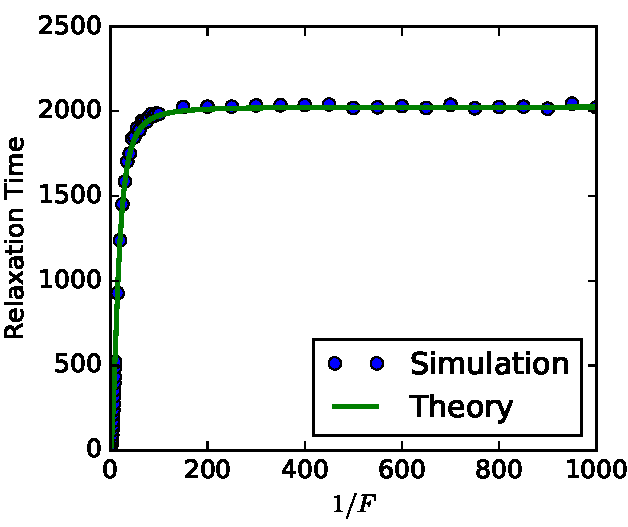
\includegraphics[width=0.8\linewidth]{relaxation1D.pdf}
    \caption{Relaxation time v.s. external force. Simulation result from 1D
        Kinetic Monte Carlo and Theory from Eq. \eqref{eq:relaxation_time_1D}
        with the setup of $\tau_0 = 1, a=1, k_B T = 1$.}
    \label{fig:relaxation1D}
\end{figure}

From Eq. \eqref{eq:time_scale} we know the estimation of time scale $\tau_0$,
but it is not a exact relation. However, we can write $\tau_0 = c\frac{2 a^2
    \xi}{k_B T}$, where $c$ is a constant. Substitute into Eq.
\eqref{eq:relaxation_time_1D} and compare the first term with Rouse theory
$\tau_{Rouse} = \frac{\xi L^2a^2}{3k_B T \pi^2}$ \cite{},  which correctly
describe the dynamics of bead rod polymer when there is no external force, we
can obtain $c=\frac{1}{12}$. Resubstitute $\tau_0$ with $c$ into Eq.
\eqref{eq:relaxation_time_1D} we obtain

\begin{equation}
    \label{eq:relaxation_time_3D}
    \tau = \frac{\xi L^2 a^2}{3 \pi^2 k_{B} T}
    - \frac{\xi L^4 a^2 \left(e^{\frac{2 F a}{k_{B} T}} - 1\right)^2}
    {3 \pi^2 k_{B} T \left(L^2 \left(e^{\frac{2 F a}{k_{B}T}} - 1\right)^2 +
            \pi^2 \left(e^{\frac{2 F a}{k_{B}T}} + 1\right)^2\right)} 
\end{equation}
This can be compared with the 3D Brownian Dynamics simulation, which is show in
Fig. \ref{fig:relaxation3D}. Notice here $L$ is the number of beads. 
\begin{figure}[htpb]
    \centering
    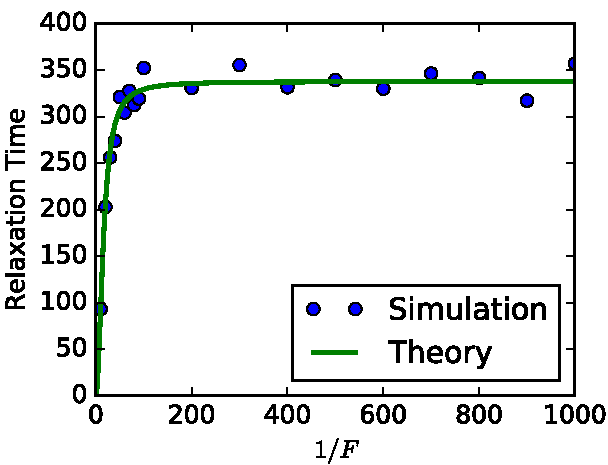
\includegraphics[width=0.8\linewidth]{relaxation3D.pdf}
    \caption{Relaxation time v.s. external force in 3D. Here the relaxation
        time of simulation is fitting from the $z$ component (force direction)
        of $\mathbf{r}_d$ (middle bead), theory is from Eq.
        \eqref{eq:relaxation_time_3D} by set $\xi=1, a=1$ and $k_B T=1$.}
    \label{fig:relaxation3D}
\end{figure}

In the mean time, we can investigate how relaxation time varies with
temperature using Eq. \eqref{eq:relaxation_time_3D}. Interestingly, in this
case, the non-monotonic behavior is predicted by the theory when external force
is strong enough, See in Fig. \ref{fig:prediction}. We don't have the simulation
data yet, but will update later on.

\begin{figure}[htpb]
    \centering
    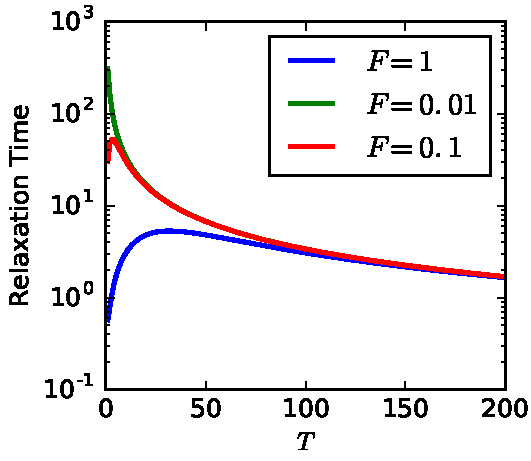
\includegraphics[width=0.8\linewidth]{prediction.pdf}
    \caption{Prediction of of theory from Eq. \eqref{eq:relaxation_time_3D} for
        how relaxation time varies with temperature.}
    \label{fig:prediction}
\end{figure}

\subsection{Equilibrium Statistics}
\label{sub:equilibrium_statistics}

Working on it...



\bibliography{report} 
\bibliographystyle{plain}
\end{document}
